%%%%%%%%%%%%%%%%%%%%%%%%%%%%%%%%%%%%

\section{Considering categorical data}

%%%%%%%%%%%%%%%%%%%%%%%%%%%%%%%%%%%%

\subsection{Contingency tables and bar plots}

%%%%%%%%%%%%%%%%%%%%%%%%%%%%%%%%%%%%

\begin{frame}
\frametitle{Contingency tables}

A table that summarizes data for two categorical variables is called a \hl{contingency table}.

$\:$ \\
\pause
The contingency table below shows the distribution of students' genders and whether or not they are looking for a spouse while in college.

\begin{center}
\begin{tabular}{l l cc rr}
					& 			& \multicolumn{2}{c}{{looking for spouse}} \\
  \cline{3-4}
					&			& No	& Yes	& Total & \hspace{3mm}  \\ 
  \cline{2-5}
\multirow{2}{*}{{gender}}& Female 		& 86 	& 51 		& 137 \\ 
  					& Male 		& 52 	& 18	 	& 70\\ 
  \cline{2-5}
  					& Total		& 138& 69	&  207 \\
  \cline{2-5}
\end{tabular}
\end{center}

\end{frame}

%%%%%%%%%%%%%%%%%%%%%%%%%%%%%%%%%%%%

\begin{frame}
\frametitle{Bar plots}

A \hl{bar plot} is a common way to display a single categorical variable. A bar plot where proportions instead of frequencies are shown is called a \hl{relative frequency bar plot}.

\begin{center}
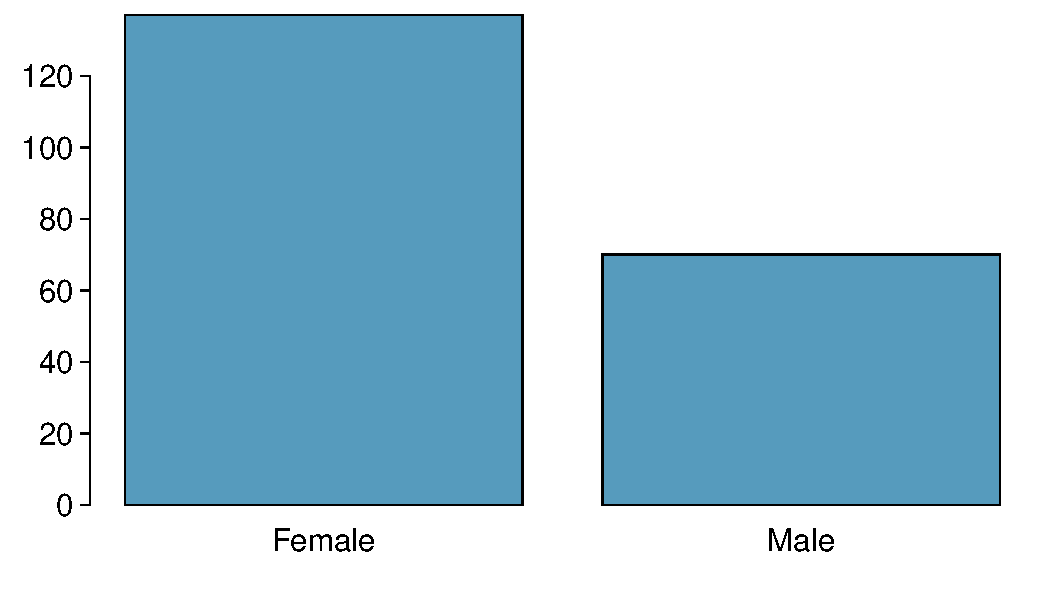
\includegraphics[width=0.45\textwidth]{1-7_categorical_data/figures/gender_spouse/gender_bar}
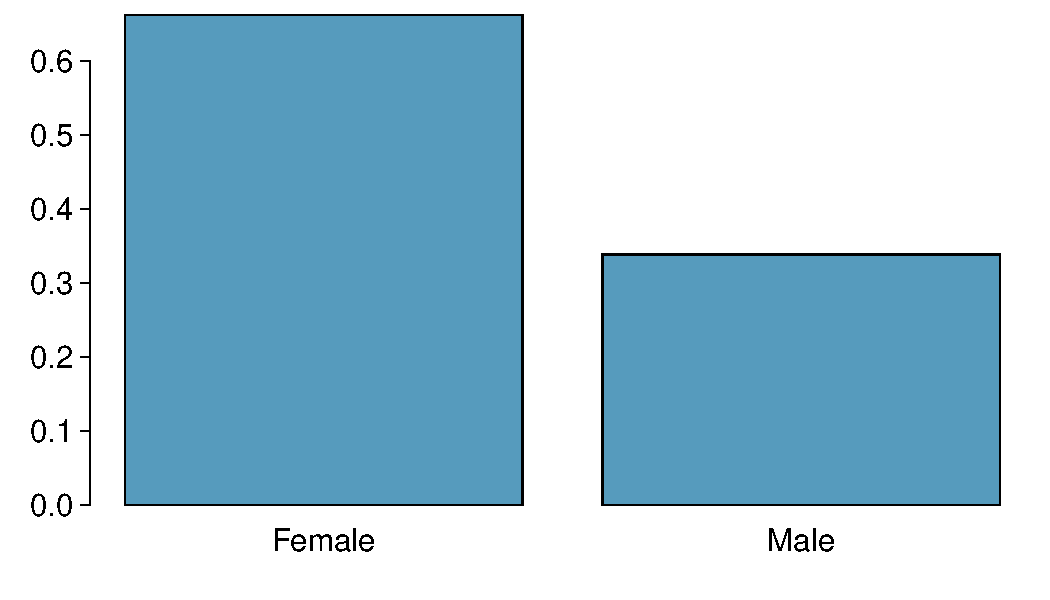
\includegraphics[width=0.45\textwidth]{1-7_categorical_data/figures/gender_spouse/gender_rel_bar}
\end{center}

\pause

\dq{How are bar plots different than histograms?}

\soln{\pause{{\scriptsize Bar plots are used for displaying distributions of categorical variables, while histograms are used for numerical variables. The x-axis in a histogram is a number line,  hence the order of the bars cannot be changed, while in a bar plot the categories can be listed in any order (though some orderings make more sense than others, especially for ordinal variables.)}}}

\end{frame}

%%%%%%%%%%%%%%%%%%%%%%%%%%%%%%%%%%

%%%%%%%%%%%%%%%%%%%%%%%%%%%%%%%%%%%%

\subsection{Row and column proportions}

%%%%%%%%%%%%%%%%%%%%%%%%%%%%%%%%%%%%

\begin{frame}
\frametitle{Choosing the appropriate proportion}

\dq{Does there appear to be a relationship between gender and whether the student is looking for a spouse in college?}

\begin{center}
\begin{tabular}{l l cc r}
					& 			& \multicolumn{2}{c}{{looking for spouse}} \\
  \cline{3-4}
					&			& No	& Yes	& Total \\ 
  \cline{2-5}
\multirow{2}{*}{{gender}}& Female 		& 86 	& 51 		& 137 \\ 
  					& Male 		& 52 	& 18	 	& 70\\ 
  \cline{2-5}
  					& Total		& 138& 69	&  207 \\
  \cline{2-5}
\end{tabular}
\end{center}

\pause

To answer this question we examine the row proportions: 

\pause

\begin{itemize}

\item \% Females looking for a spouse: $51 / 137 \approx 0.37$ \\

\pause

\item \% Males looking for a spouse: $18 / 70 \approx 0.26$ \\

\end{itemize}

\end{frame}

%%%%%%%%%%%%%%%%%%%%%%%%%%%%%%%%%%%%

\subsection{Segmented bar and mosaic plots}

%%%%%%%%%%%%%%%%%%%%%%%%%%%%%%%%%%%%

\begin{frame}
\frametitle{Segmented bar and mosaic plots}

\dq{What are the differences between the three visualizations shown below?}

\begin{center}
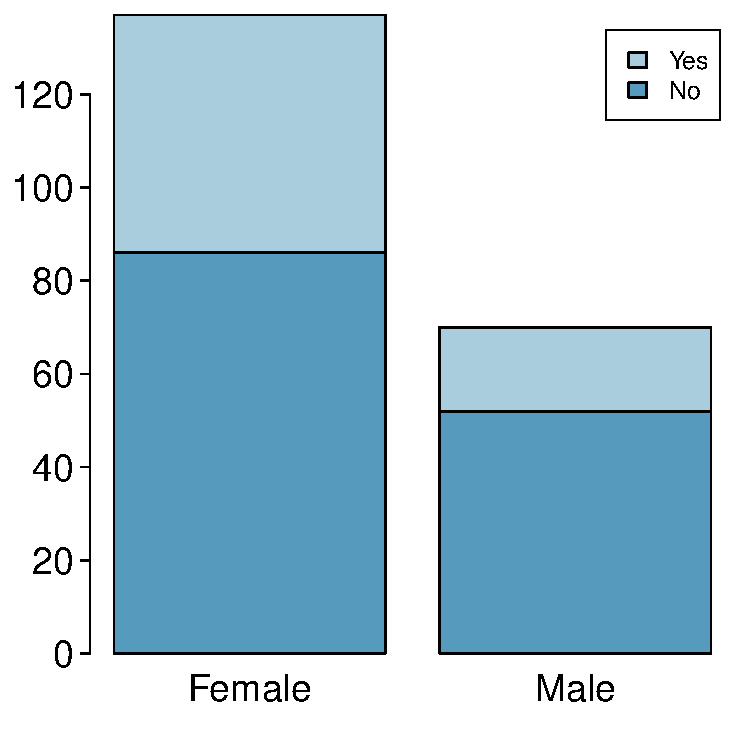
\includegraphics[width=0.33\textwidth]{1-7_categorical_data/figures/gender_spouse/gender_seg_bar}
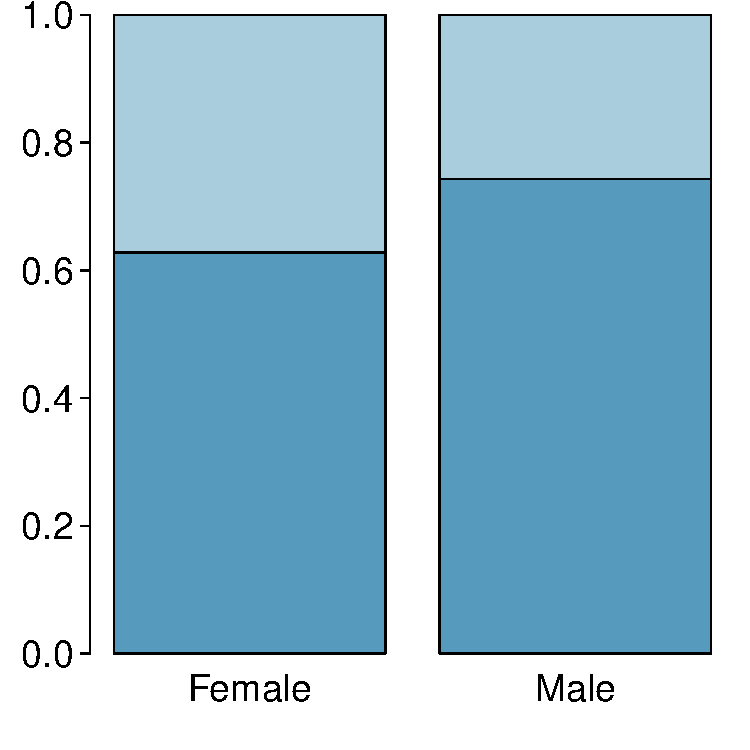
\includegraphics[width=0.33\textwidth]{1-7_categorical_data/figures/gender_spouse/gender_rel_seg_bar}
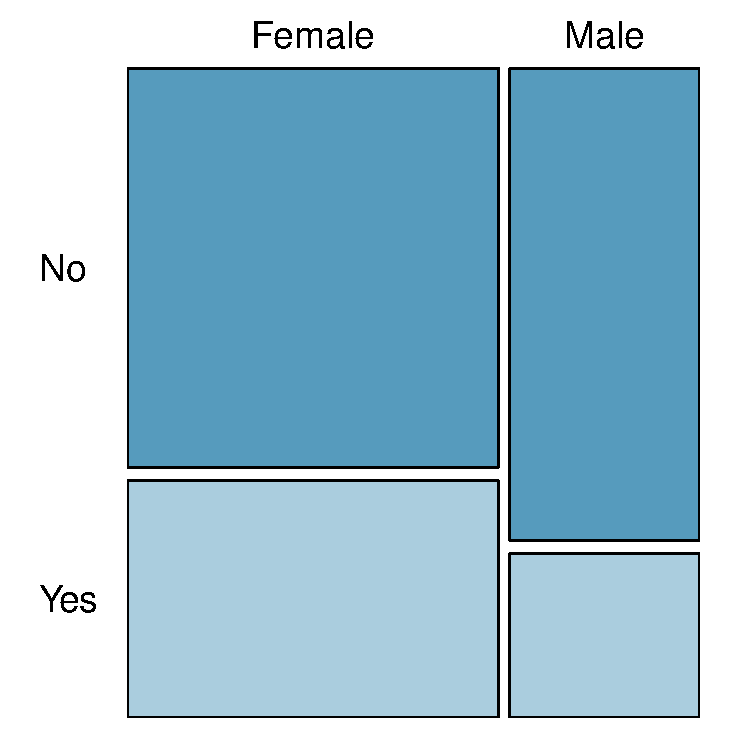
\includegraphics[width=0.33\textwidth]{1-7_categorical_data/figures/gender_spouse/gender_mosaic}
\end{center}

\end{frame}

%%%%%%%%%%%%%%%%%%%%%%%%%%%%%%%%%%%%

\subsection{Pie charts}

%%%%%%%%%%%%%%%%%%%%%%%%%%%%%%%%%%%%

\begin{frame}
\frametitle{Pie charts}

\dq{Can you tell which order encompasses the lowest percentage of mammal species?}

\vspace{-0.5cm}

\begin{center}
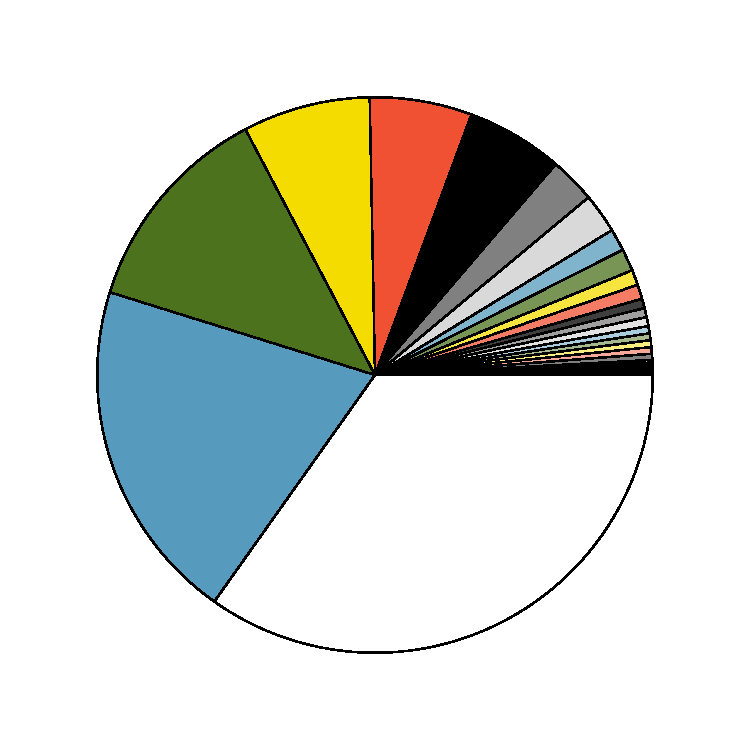
\includegraphics[width=0.4\textwidth]{1-7_categorical_data/figures/mammal_pie_chart/mammal_pie_chart}
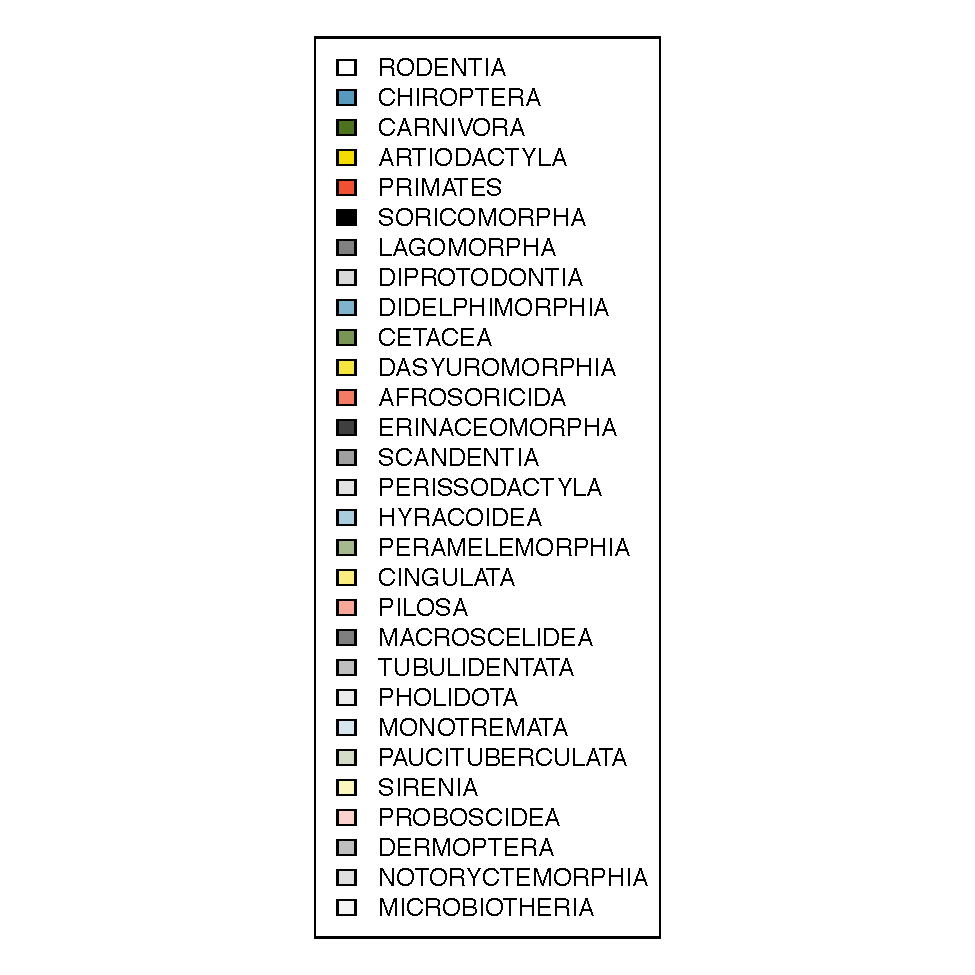
\includegraphics[width=0.2\textwidth]{1-7_categorical_data/figures/mammal_pie_chart/mammal_pie_chart_legend}
\end{center}

\ct{Data from \webURL{http://www.bucknell.edu/msw3}.}

\end{frame}


%%%%%%%%%%%%%%%%%%%%%%%%%%%%%%%%%%%%

\subsection{Comparing numerical data across groups}

%%%%%%%%%%%%%%%%%%%%%%%%%%%%%%%%%%%%

\begin{frame}
\frametitle{Side-by-side box plots}

\dq{Does there appear to be a relationship between class year and number of clubs students are in?}

\begin{center}
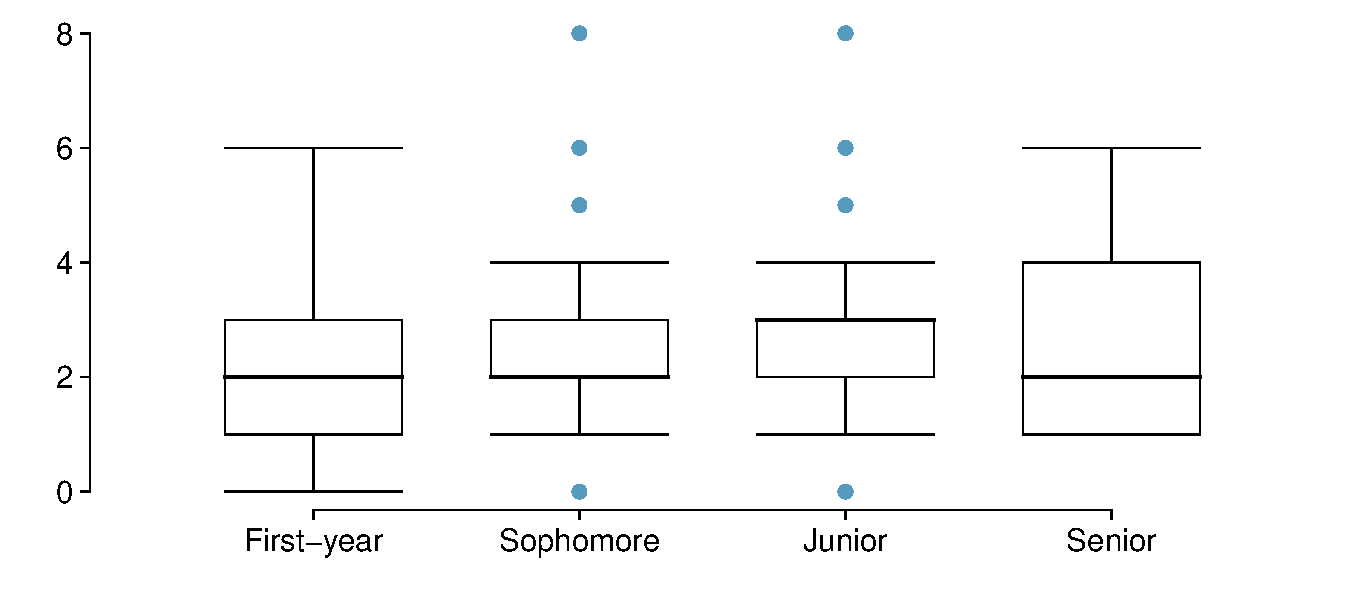
\includegraphics[width=\textwidth]{1-7_categorical_data/figures/year_clubs/year_clubs}
\end{center}

\end{frame}

%%%%%%%%%%%%%%%%%%%%%%%%%%%%%%%%%%%%

